\begin{figure}[!h]
\centering
\begin{subfigure}[b]{1.0\textwidth}
\centering
	%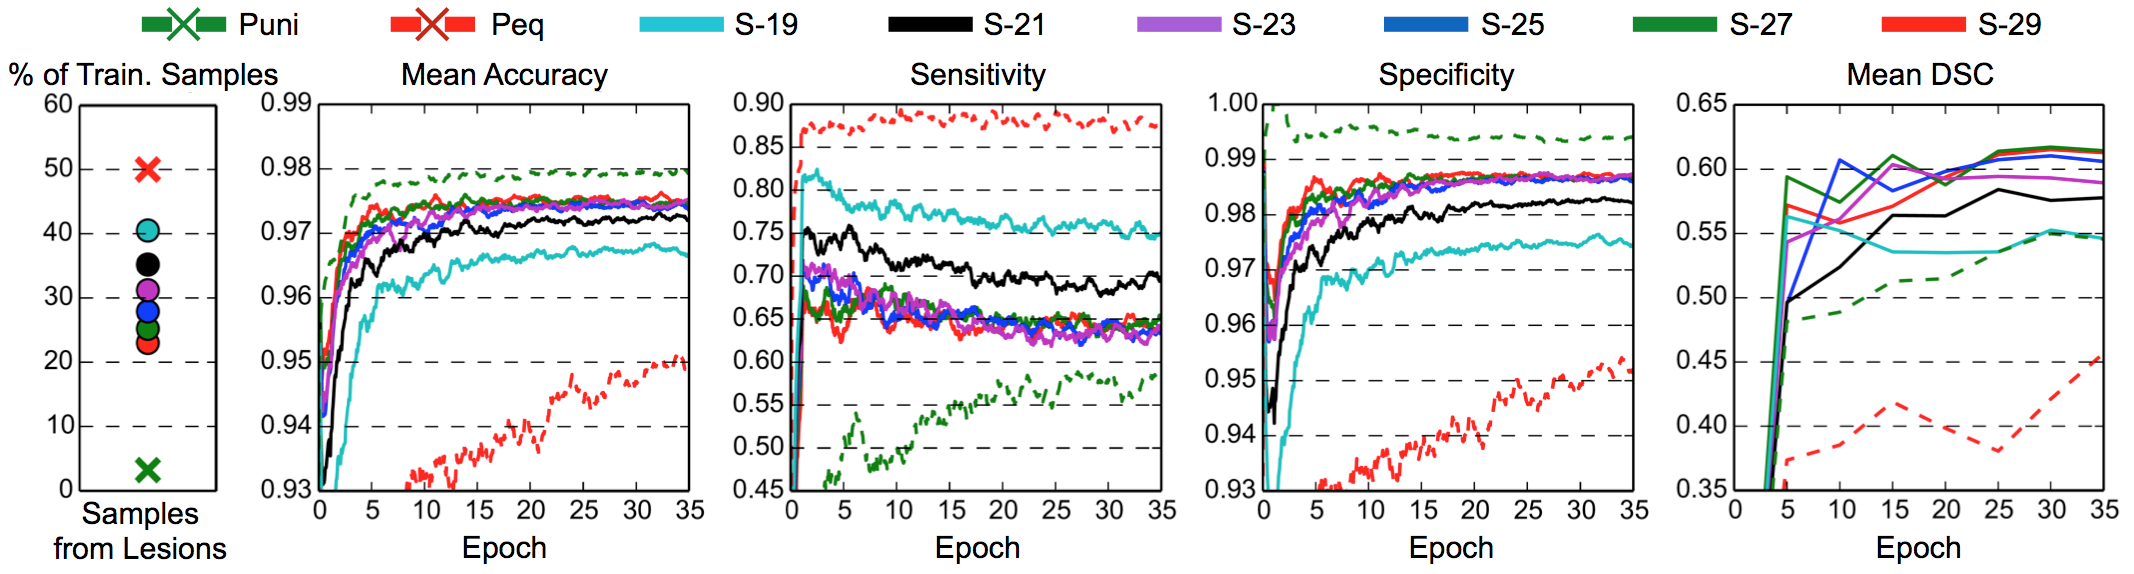
\includegraphics[clip=true, trim=10pt 270pt 30pt 210pt, width=1.0\textwidth]{figures/validationOfArchitecture/denseTraining/denseFigureToPlace.pdf}
	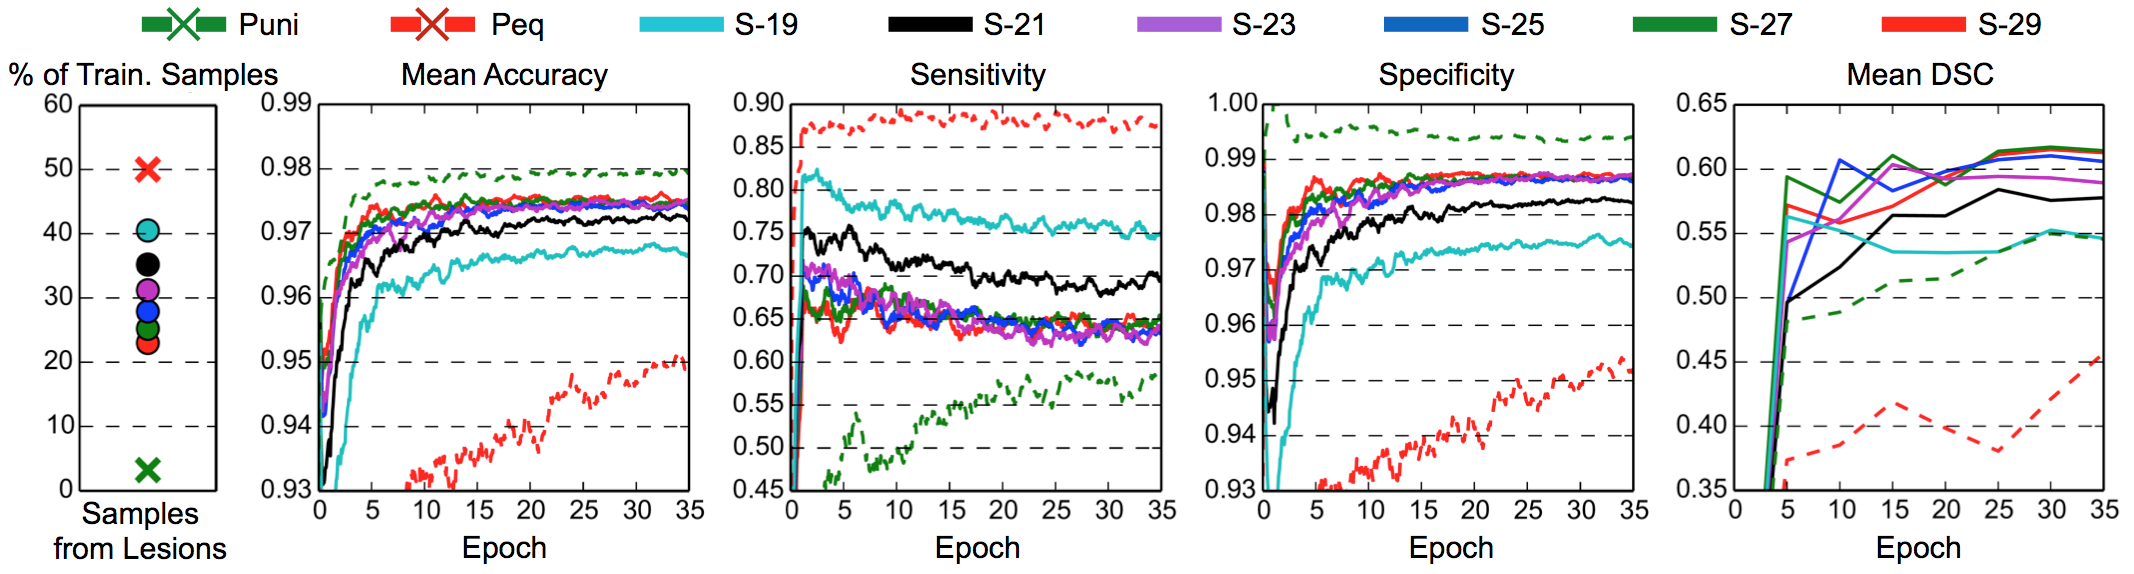
\includegraphics[clip=true, trim=0pt 0pt 0pt 0pt, width=1.0\textwidth]{figures/validationOfArchitecture/denseTraining/denseFigureToPlace.png}
\end{subfigure}
\caption{Comparison of the commonly used methods for training on patches uniformly sampled from the brain region (P$_\text{uni}$) and equally sampled from lesion and background (P$_\text{eq}$) against our proposed scheme (S-${d}$) on cubic segments of side length $d$, also equally sampled from lesion and background. We varied $d$ to observe its effect. From left to right: percentage of training samples extracted from the lesion class, mean accuracy, sensitivity, specificity calculated on uniformly sampled validation patches and, finally, the mean DSC of the segmentation of the validation datasets. The progress throughout training is plotted. Because lesions are small, P$_\text{uni}$ achieves very high voxel-wise accuracy by being very specific but not sensitive, with the opposite being the case for P$_\text{eq}$. Our method achieves an effective balance between the two, resulting in better segmentation as reflected by higher DSC.}
\label{fig:denseTrainingExperiment}
\end{figure}
%\vspace{-1pt} %takes away some white space before figure